\documentclass{article}
% translate with >> pdflatex -shell-escape <file>

% This file is used as unit test for pgfplots, copyright by Christian Feuersaenger.
% 
% See
%   http://pgfplots.sourceforge.net/pgfplots.pdf
% for pgfplots.
%
% Any required input files (for <plot table> or <plot file> or the table package) can be downloaded
% at
% http://www.ctan.org/tex-archive/graphics/pgf/contrib/pgfplots/doc/latex/
% and
% http://www.ctan.org/tex-archive/graphics/pgf/contrib/pgfplots/doc/latex/plotdata/

\usepackage{pgfplots}
\pgfplotsset{compat=newest}

\pagestyle{empty}

\begin{document}
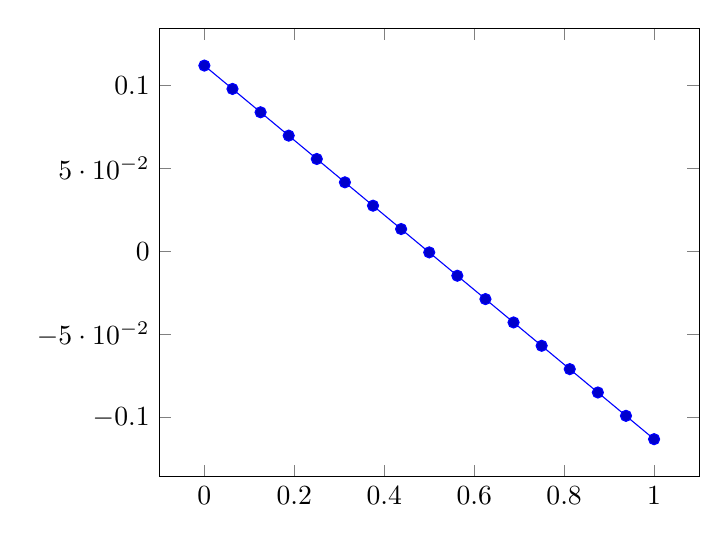
\begin{tikzpicture}%
\begin{axis}

\addplot plot coordinates {
	(0.000000,	0.112104)
	(0.062500,	0.098029)
	(0.125000,	0.083954)
	(0.187500,	0.069879)
	(0.250000,	0.055804)
	(0.312500,	0.041729)
	(0.375000,	0.027654)
	(0.437500,	0.013579)
	(0.500000,	-0.000496)
	(0.562500,	-0.014571)
	(0.625000,	-0.028646)
	(0.687500,	-0.042722)
	(0.750000,	-0.056797)
	(0.812500,	-0.070872)
	(0.875000,	-0.084947)
	(0.937500,	-0.099022)
	(1.000000,	-0.113097)
};
\end{axis}
\end{tikzpicture}
\end{document}
